\chapter{Architecture robotique}
\label{chap:integration}

\epigraph{\foreignlanguage{USenglish}{The belief that complex systems
    require armies of designers and programmers is wrong. A system
    that is not understood in its entirety, or at least to a
    significant degree of detail by a single individual, should
    probably not be built.}}{Niklaus Wirth}
\clearpage

\lettrine[lines=2, lraise=0.1, nindent=0em, slope=-.5em]%
{C}{e} chapitre est dédié à la conception d'architectures robotiques
complexes permettant la validation de nouveaux algorithmes robotiques.
Les précédents chapitres ont montré une progression d'une approche qui
est dédiée purement à la génération de trajectoires par l'utilisation
d'outils d'optimisation numérique vers l'exécution de scénarii
dont la complexité a augmentée incrémentalement. Ce passage de la
génération de trajectoire sans ``conscience'' de ce qu'est un système
évoluant dans le monde réel vers une application robotique réelle ne
va pas sans la nécessité d'intégrer et de maîtriser une grande variété
d'algorithmes et de technologies tout en les utilisant conjointement
afin de finalement, atteindre un objectif de haut niveau. Ce chapitre
va donc décrire l'architecture qui a été mise en place sur le robot
humanoïde HRP-2\index{HRP-2} afin de réaliser un ensemble de scénario
expérimentaux, certains faisant partie intégrante des chapitres
précédents et d'autres étant le résultat de travaux de recherche
disjoints, mais prenant appui sur l'architecture développée ici. Ce
chapitre tente également de fournir des conseils et une méthodologie
pour la conception d'applications robotiques.

\section{Architecture}


Les systèmes robotiques peuvent être décomposés en trois grandes
parties:

\begin{enumerate}
\item La couche de perception\index{perception} qui analyse
  l'environnement autour du robot et construit un modèle du monde,
\item La couche de décision\index{décision} qui va tenter de résoudre
  la tâche donnée au système tout en prenant en compte l'état actuel
  du monde,
\item La couche action\index{action} qui va utiliser les capacités du robot pour
  réaliser la tâche proprement dite. En particulier, les capacités
  d'actionnement du robot sont ici utilisées pour impacter le monde
  environnant.
\end{enumerate}


Cette architecture largement décrite par la littérature est encore
d'actualité pour les robots humanoïdes. En effet, cette catégorisation
est issue de la présence dans un système robotique de boucles lentes
et de boucles rapides. Typiquement, la prise de décision est un
processus lent -- qui peut prendre plusieurs secondes --, la
planification de mouvements est un exemple de ce type de processus. Au
contraire, la couche action contrôlant les actionneurs nécessite le
plus souvent d'être extrêmement réactive et impose des contraintes
importantes en terme de temps réel. Il faut pouvoir garantir que la
boucle de contrôle peut être évaluée à une fréquence donnée ce qui
contraint à la fois le type d'algorithmes pouvant être exécuté dans
cette boucle ainsi que le volume de données pouvant être traité. Enfin,
la couche de perception est, elle, en général plus lente que le
contrôle et dépendante de la vitesse à laquelle les capteurs du robot
peuvent fonctionner. Qui plus est, il arrive parfois que les capteurs
acquièrent des données plus vite qu'elles sont traitées et certaines
données sont alors ignorées silencieusement. On a donc ici trois types
de comportements extrêmement différents.


Les couches perception et décision nécessitent une grande puissance de
calcul pour pouvoir assurer une réactivité suffisante. Cette puissance
de calcul est parfois déportée sur un ordinateur spécifique. Par
exemple dans le cadre du robot HRP-2, deux ordinateurs sont
embarqués. Le premier est dédié à la boucle de contrôle temps réel et
est relié aux actionneurs tandis que le second est relié aux capteurs
-- ici les caméras embarquées -- et supporte les algorithmes de
décision et de perception.


Afin de découpler les algorithmes robotiques, chaque algorithme est
implémenté au sein d'un composant robotique\index{composant
  robotique}\index{n\oe ud|see{composant robotique}}. En pratique, un
composant robotique est un processus -- c'est-à-dire un programme
indépendant -- pouvant communiquer avec un ou plusieurs autres
composants. La distribution des calculs sur plusieurs ordinateurs rend
nécessaire la définition d'un protocole de transmission des données
afin de pouvoir assurer une bonne interprétation de ces dernières au
sein d'un environnement informatique hétérogène. Un exemple est la
représentation des nombres au sein des architectures informatiques:
une architecture peut être dit ``big endian''\index{big endian
  (architecture)} ou ``little endian''\index{little endian
  (architecture)} selon l'ordre dans lequel les bits représentants le
nombre sont enregistrés. Dans une architecture ``big endian'' les
bits ayant les poids les plus forts sont contenus en mémoire en
premier tandis que les architectures ``little endian'' adoptent un
ordre inverse. Ce type de problème rend nécessaire la définition d'un
modèle de communication entre composants.


Les architectures robotiques autorisent généralement la communication
entre deux composants, ou n\oe uds, soit sous une forme discrète, soit
sous une forme continue. La forme discrète est appelée
``service''\index{service} et se modélise sous la forme d'un appel de
fonction distant. Un algorithme est généralement divisé en fonctions,
ces dernières formant des blocs logiques pouvant être combinés entre
eux pour réaliser des comportements de plus haut niveau. Les services
fournissent un moyen d'appeler une fonction qui sera non pas exécutée
au sein du processus courant, mais dans un autre processus, voire sur
un autre ordinateur de manière transparente. La difficulté résidant
dans le passage des arguments et la transmission du résultat. Il est
nécessaire que cette fonction soit définie selon des règles
particulières afin de s'asssurer que les données peuvent être
correctement transmises via le réseau sans compromettre leur
intégrité. Cette phase, dite de
``sérialisation''\index{sérialisation}, assure le fonctionnement de
ces mécanismes dans des environnements informatiques hétérogènes. La
seconde forme de communication sert à modéliser des flux de données
continus et est appelée ``topic''\index{topic}. Dans ce cas, le
premier composant communique à un ou plusieurs autres des données
mises à jour régulièrement. De la même façon, un processus de
sérialisation est nécessaire pour assurer que les données peuvent être
transmises même si un ou plusieurs autres composants ne font pas
partie du même processus ou ne sont pas exécutés sur le même
ordinateur.


De nombreux outils logiciels implémentent ces mécanismes sous
différentes formes. Le choix réalisé sur le robot humanoïde HRP-2 a
été d'utiliser ROS -- Robotics Operating System --\index{ROS}, un
projet communautaire initié par la société californienne Willow
Garage\index{Willow Garage}. Le mécanisme de communication ainsi
qu'une grande partie de la modélisation du processus de perception se
fonde sur les outils développés dans le cadre de ce projet. Les
sections suivantes vont détailler les différents composants
fonctionnant sur le robot humanoïde HRP-2\index{HRP-2}.



\subsection{Contrôle}

Sous le terme de ``contrôle'' est désigné le composant robotique
chargé de calculer la commande qui sera envoyée aux actionneurs. Il
est impératif que cet ordre déterminant le prochain état que les
servomoteurs du système vont s'efforcer d'atteindre soit envoyé à une
fréquence fixe. Sur le robot humanoïde HRP-2\index{HRP-2}, la
fréquence de la boucle de contrôle est de 200$\hertz$, il faut donc
que la boucle de contrôle ne mette pas plus de 5ms pour être
évaluée. Les noyaux des systèmes d'exploitation multitâches ne
fournissent pas de garantie forte sur la réactivité des logiciels
exécutés. Il est donc nécessaire d'utiliser des noyaux dédiés afin
d'assurer que la boucle de contrôle soit exécutée en permanence à la
fréquence voulue. Ces contraintes impliquent que les composants de
contrôle se doivent d'être aussi minimaux que possible et sont souvent
monolithiques. À ce sujet, les contrôleurs robotiques partagent une
grande ressemblance avec les noyaux des systèmes d'exploitation. Ils
assurent également la sûreté du système: une mauvaise commande envoyée
aux moteurs peut, très facilement, entraîner la destruction des
actionneurs.

Dans le cas de systèmes robotiques complexes, il est courant d'avoir
plusieurs contrôleurs exécutés successivement au sein de la boucle de
contrôle. Ainsi l'architecture d'HRP-2 se fonde sur un système de
plug-in permettant de charger des contrôleurs ``à chaud''. Chaque
contrôleur est alors modélisé par une machine à état très simple
illustrée par la \autoref{fig:controleur}. Le contrôleur passe alors
par les états suivants:

\begin{itemize}
\item Initialisation sans contrainte de temps réel.
\item Initialisation avec contrainte de temps réel.
\item Exécution.
\item Destruction avec contrainte de temps réel.
\item Destruction sans contrainte de temps réel.
\end{itemize}

\begin{figure}
  \begin{center}
    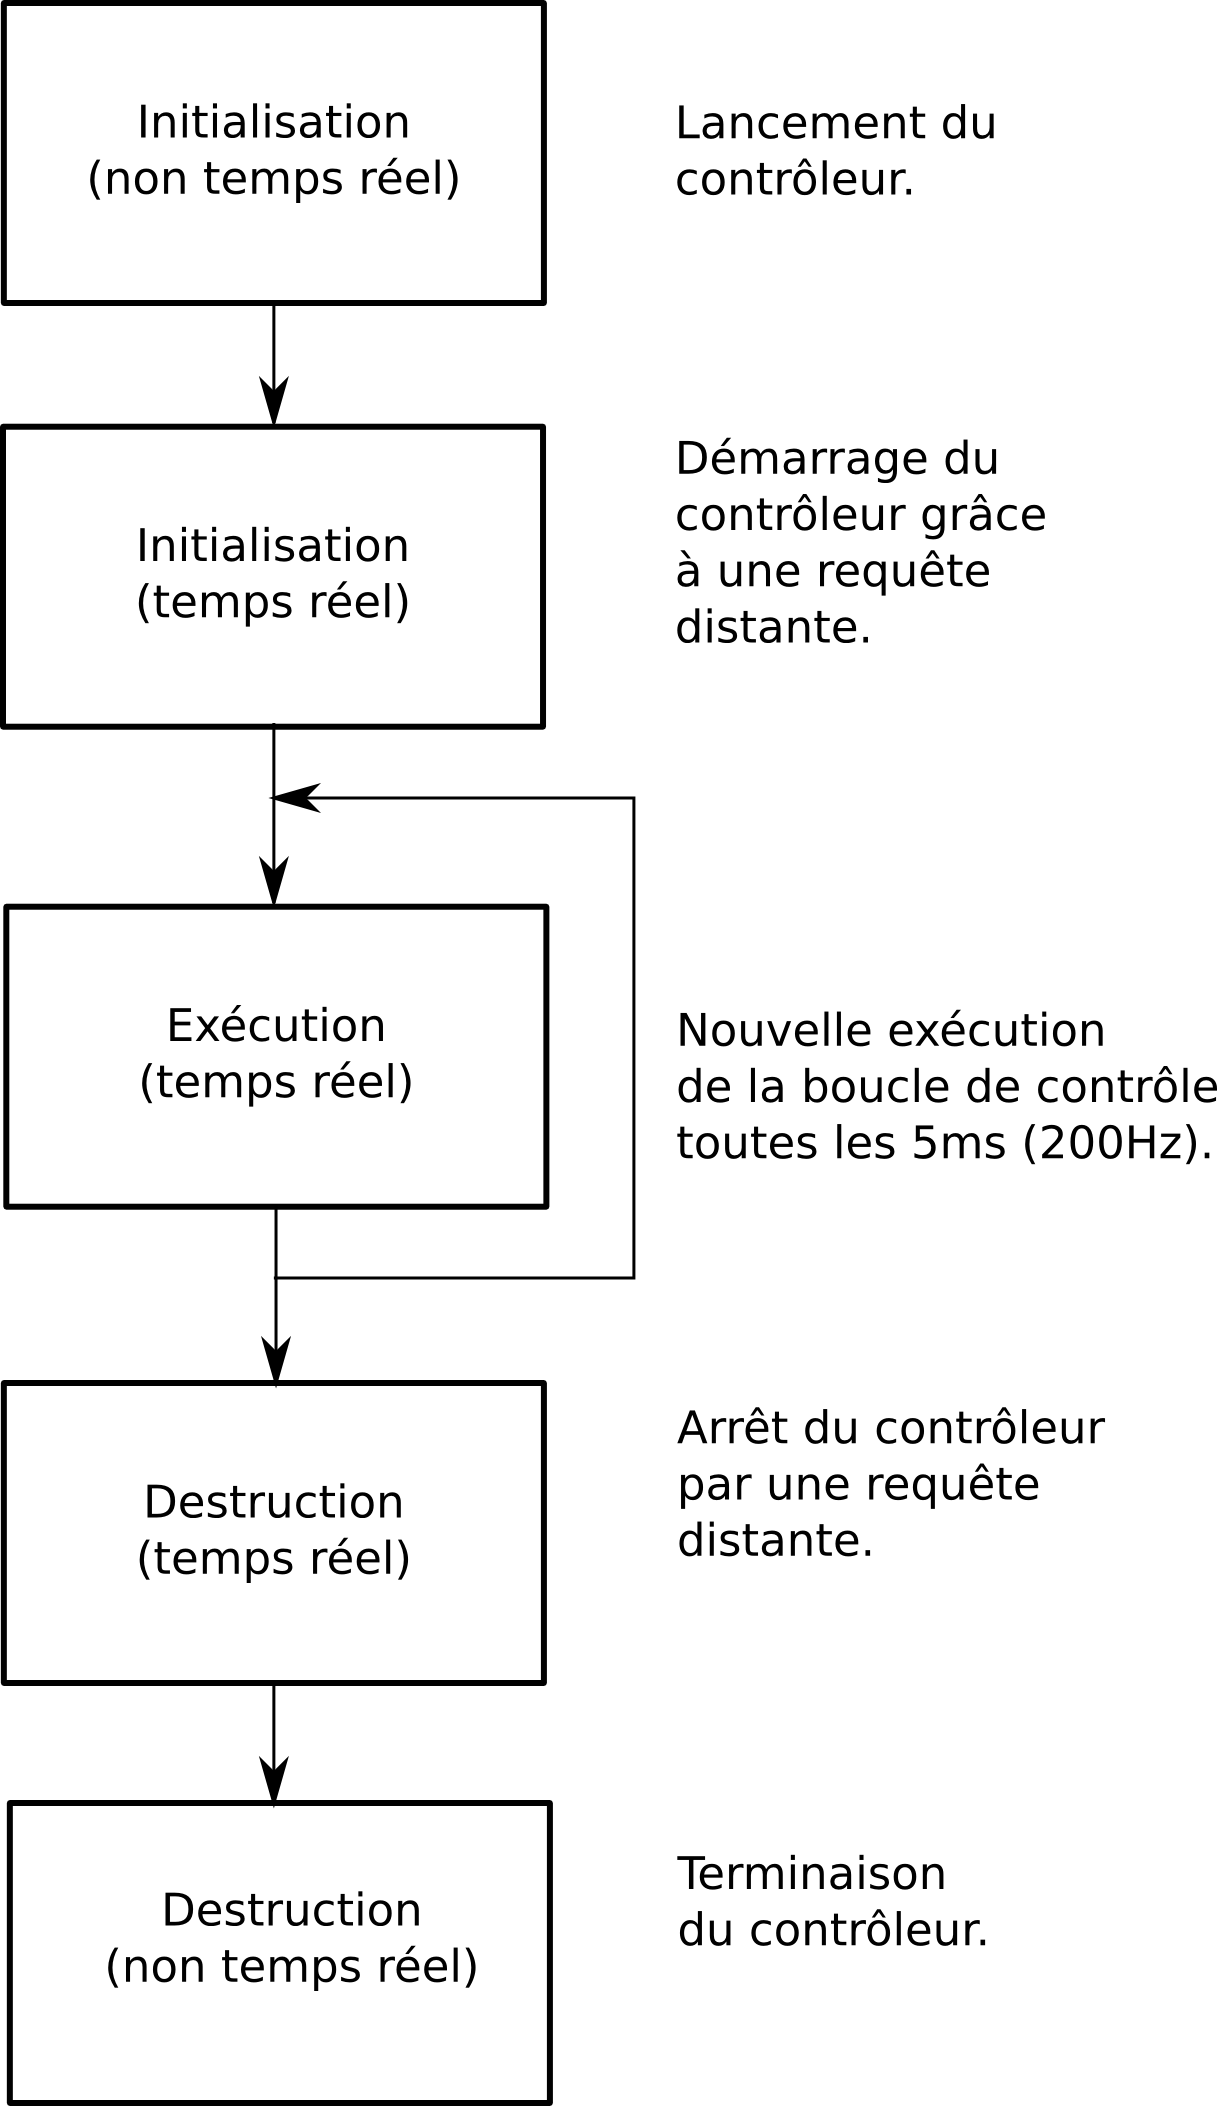
\includegraphics[width=.9\linewidth]{src/chap4-integration/controleur.png}
  \end{center}
  \caption{Schéma de fonctionnement d'un contrôleur temps
    réel. Plusieurs contrôleurs de ce type peuvent être lancés. Dans
    ce cas, chaque tour de la boucle de contrôle correspond à une
    exécution de la boucle de contrôle de chaque contrôleur actif --
    initialisé -- dans l'ordre dans lequel ils ont été créés. \label{fig:controleur}}
\end{figure}

Le passage d'un état à l'autre se réalisant dans l'ordre, avec un
bouclage sur la phase d'exécution autant qu'il soit nécessaire.


L'architecture de contrôle est divisée en trois contrôleurs:
\begin{description}
\item[Pile de tâches.\index{pile de tâches}] À partir d'un ensemble de
  tâches, la résolution de la pile de tâches est calculée dans la
  boucle de contrôle afin de calculer la commande à envoyer aux
  moteurs. HRP-2 étant commandé en position, la commande envoyée
  correspond à la position articulaire des différents articulations du
  système.
\item[Stabilisateur.\index{stabilisateur}] HRP-2 intègre un mécanisme
  d'absorption passif des chocs appelé ``silent blocs''\index{silent
    block}. Ce système passif intègre au niveau des chevilles une
  compliance difficile à modéliser et à prendre en compte dans le
  calcul de la commande. La centrale inertielle du robot permettant
  d'estimer l'attitude du bassin, le stabilisateur peut déduire
  l'état des flexibilités des chevilles et, à l'aide des capteurs de
  force placés dans les chevilles, réaliser un asservissement
  bas-niveau sur la trajectoire du ZMP\index{Zero-Momentum Point}
  désiré. Ce mécanisme permet de compenser la modélisation sommaire de
  la dynamique réalisée, par exemple, par l'utilisation du modèle
  simplifié du ZMP ainsi que des éventuelles erreurs de modélisation
  de la structure du robot. Ce système compense les erreurs de suivi
  du ZMP en modifiant les valeurs des articulations des jambes du
  robot.
\item[Communication.] Le dernier élément communique vers l'extérieur
  les informations liées au contrôle du robot tel que les commandes
  envoyées, réellement exécutées -- c'est-à-dire après stabilisation
  --, ainsi que les sorties des capteurs tels que la centrale
  inertielle et les capteurs de force placés aux chevilles et poignets
  du robot.
\end{description}


On notera que pour le dernier contrôleur, la communication réseau
étant implémentée en TCP/IP\index{TCP/IP}, il n'est pas possible de
garantir le temps pris par l'envoi des données et il est donc
impossible d'envoyer des données en TCP/IP\index{TCP/IP} sans
compromettre la boucle temps réel. Cette partie est donc divisée en
plusieurs fils d'exécution non bloquants afin de garantir la sûreté du
système. En pratique, chaque ``topic'' permettant la communication de
données vers l'extérieur publie les données dans un fil d'exécution
séparé et non temps réel. Le fil d'exécution\index{fil d'exécution}
temps réel lui tente de copier la donnée vers une variable lue par ce
fil d'exécution. Si ce dernier est en train d'y accéder et qu'elle
n'est pas accessible, un verrou protège l'accès à la ressource et la
publication de la donnée pour ce tour de boucle est ignorée. En
pratique, la communication vers l'extérieur est réalisée à 20$\hertz$. En
moyenne, une donnée sur dix est donc envoyée afin d'éviter d'engorger
le système.


En terme de conception, les composants nécessitant un rafraichissement
à une vitesse supérieure doivent être intégrés à la boucle de
contrôle. Pour les autres données, il faut pouvoir, via le schéma de
calcul, utiliser les informations temporelles attachées aux
données capteur envoyées pour gérer de manière consistante le retard
inhérent à toute donnée provenant d'une architecture distribuée.


\subsection{Vision}


La vision\index{vision robotique} est l'élément central de la
perception sur un robot humanoïde. Elle est caractérisée par une
particularité qui détermine tous les traitements qui lui sont
affectés: les caméras produisent des quantités de données extrêmement
importantes. De ce fait, il est important d'éviter de réaliser des
traitements inutiles et il faut également éviter au maximum les
copies. Le traitement des images est souvent réalisé en série: on
acquiert une image, on la convertit, on la rectifie et puis on cherche
à en tirer des informations de plus haut niveau. Ces traitements en
série se modélisent particulièrement bien sous la forme d'un tuyau
dans lequel les images passent les unes après les autres. La stratégie
classique de la robotique tend alors à dédier un composant par
traitement afin de garder un système modulaire, mais la taille des
données rend cela difficile. En effet, si chaque composant vit dans un
processus différent, il est nécessaire de passer par des mécanismes de
mémoire partagée afin d'éviter les copies en mémoire. ROS a choisi une
seconde stratégie en offrant la possibilité d'agglomérer plusieurs
composants dans un seul processus\footnote{L'agrégation de plusieurs
  n\oe uds se nomme ``nodelet'':
  \url{http://ros.org/wiki/nodelet}.}. La sérialisation devient donc
totalement inutile au prix d'une plus grande complexité dans
l'écriture des n\oe uds et d'une forme d'insécurité: si un problème
advient dans n'importe lequel de ces composants, il provoquera l'arrêt
de la totalité du système. Cependant, les traitements étant effectués
en série, devoir relancer tous les traitements en cas de panne n'amène
pas de perte significative de qualité de service.


Nous allons donc désormais nous attacher à développer les différents
composants de vision qui ont été utilisés sur le robot
HRP-2\index{HRP-2} et agglomérés dans la chaîne de traitement des
images du robot.


\paragraph{Acquisition des images}

L'acquisition des images est réalisée par un composant communiquant
avec le pilote FireWire. Les quatre caméras du robot sont des Flea2 du
fabricant PointGrey. Ces caméras sont reliées à un FireWire IEEE
1394b\index{FireWire IEEE 1394b}. Les limitations du bus ne permettent
pas l'acquisition des données sur les quatre caméras simultanément, on
peut donc passer de la paire de caméras grand-angle à la seconde paire
de caméras. La première paire est dédiée à la perception de
l'environnement au détriment de la précision tandis que la seconde
dispose d'un champ plus resserré, adapté à la manipulation fine
d'objets notamment.

Les images acquises utilisent un encodage de Bayer\index{Bayer
  (encodage de)}. Cet encodage, nommé du nom de son inventeur, Bryce
E. Bayer chercheur au sein de la société Kodak, réalise l'encodage
d'images couleurs sur 8 bits au lieu des 24 bits habituellement
nécessaires pour représenter les trois canaux utilisés pour encoder
les trois couleurs primaires: rouge, vert et bleu. Cet encodage encode
la couleur verte sur 50\% du volume de données totale tandis que bleu
et rouge représentent 25\% chacun. Cette prépondérance du vert est
fondée sur la plus grande sensibilité au vert des cônes, les
photorécepteurs présents au fond de l'\oe il.


\paragraph{Traitements des images}

Une fois les images acquises, il est important de les convertir dans
un espace colorimétrique\index{espace colorimétrique} adapté à leur
traitement. La première étape est donc de dématricer les images
encodées en Bayer vers des images monochromatiques ou couleurs 24 bits
dans l'espace RGB habituel. Dès maintenant, un branchement s'effectue
entre les traitements utilisant les images couleur et les traitements
utilisant les informations de luminance uniquement. Afin de fournir
une expérience unifiée, les deux ``topics'' sont créés, mais les
traitement ne sont effectués qu'à partir du moment où au moins un
client se connecte à ce dernier. On peut donc offrir une large palette
de possibilités sans mettre à mal les performances du système. Le
dématriçage\index{dématriçage} des images encodées en Bayer
reconstruit les couleurs manquantes en interpolant grâce à la couleur
des pixels adjacents. Plusieurs techniques ayant des coûts de calcul
différents existent selon les cas: interpolation bilinéaire,
interpolation bicubique ou bien encore rééchantillonage de
Lanczos\index{Lanczos (rééchantillonage de)}.


La seconde étape consiste à rectifier les images. Nous nous
intéresserons d'abord au cas de la rectification\index{rectification}
monoculaire. Dans ce cas, l'objectif de ce procédé est de se ramener
au cas de la caméra parfaite dit
``pinhole''\index{sténopé}\index{modèle de caméra
  pinhole|see{sténopé}} -- ou sténopé en français -- où la projection
du point 3D $P$ sur le plan image donne un point 2d $p$ qui correspond
parfaitement à la projection de ce dernier en passant par le point
focal de la caméra $C$: $p_x = P_x / P_z$ et $p_y = P_y / P_z$ où
$P_x, P_y, P_z$ sont les coordonnées du point dans l'espace 3D et
$p_x, p_y$ les coordonnées 2D du point $p$ dans le plan image. Ce
n'est pas jamais totalement le cas en réalité: le plan image n'est pas
un plan parfait, l'axe optique n'est jamais exactement au centre de la
caméra et les objectifs réalisent une distorsion\index{distorsion} des
rayons lumineux captés. Pour pouvoir raisonner sur ce modèle idéal, on
va donc traiter l'image afin qu'elle puisse être considérée comme
provenant d'un capteur idéal ayant le comportement d'un sténopé, à la
différence de la caméra réelle. Il faut pour cela calibrer la caméra
et identifier ses paramètres intrinsèques\index{paramètres
  intrinsèques (de caméra)}: $(u_0, v_0)$ la position de l'axe optique
dans l'image, $(p_x, p_y)$ la taille des pixels permettant de réaliser
la conversion des pixels vers les mètres et un ensemble de paramètres
permettent d'identifier la distorsion de l'image originale. Plusieurs
modèles sont décrits par la littérature, mais dans notre cas une
estimation de la distorsion radiale\index{distorsion radiale} est
suffisante pour compenser l'utilisation d'un objectif grand-angle.


Le processus de calibration\index{calibration (d'une caméra)} est
réalisé en utilisant une mire que l'on place à différents endroits
relativement à la caméra. Connaissant la taille des points et leur
écartement, on peut alors, par la résolution d'un problème type
moindres carrés linéaire, réaliser une estimation des paramètres
intrinsèques des caméras du système.

Une fois de plus, ce traitement est disponible dans deux variantes
différentes: monochromatique et couleur.

\begin{figure}
  \begin{center}
    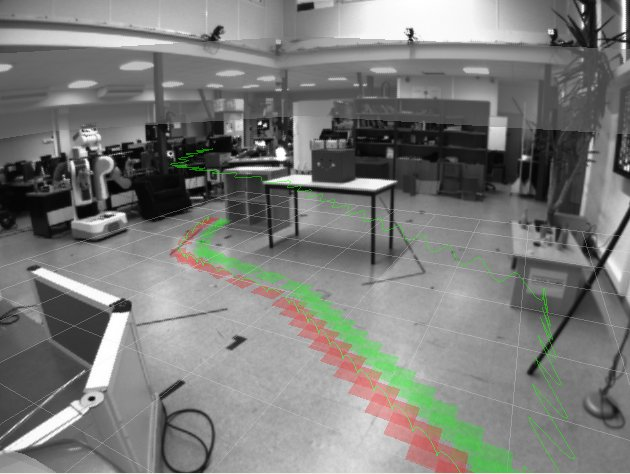
\includegraphics[width=.95\linewidth]{src/chap4-integration/footsteps2.jpg}
  \end{center}
  \caption{Affichage de la pile de pas que le robot va réaliser en
    réalité augmentée.}
\end{figure}



\paragraph{Vision stéréoscopique}\index{vision stéréoscopique}


Le dernier traitement concernait la vision monoculaire. Il est
courant, en robotique, d'avoir recours à la vision stéréoscopique afin
de pouvoir reconstruire la profondeur d'un objet visible dans les deux
caméras. Il est alors nécessaire d'estimer la transformation relative
entre les deux caméras afin de pouvoir rectifier l'image de la seconde
image de la paire de caméras stéréo. Une fois ce processus effectué,
on peut estimer que les images de deux caméras ont été prises par des
capteurs virtuels dont les plans images sont coplanaires. On peut
alors faire en sorte que la projection d'un point 3D se fasse sur la
même ligne tant sur la caméra de gauche que sur la caméra de
droite. Le problème de l'appariement des points se ramène alors à un
problème unidimensionnel de complexité moindre permettant la
construction d'une carte de profondeur. Cette carte est disponible
sous la forme d'un topic, mais les données de profondeur sont
également disponibles sous la forme d'un nuage de points. Dans ce
dernier, on associe à chaque point la couleur du pixel correspondant
dans l'image. Ce topic est particulièrement utile lorsque l'on
souhaite utiliser des algorithmes de traitements de nuages de
points 3D tels que PCL -- la Point Cloud Library --\index{PCL (Point
  Cloud Library)}.


Une fois de plus, la totalité du processus de vision peut fonctionner
dans un processus unique afin d'éviter les copies. Cette architecture,
également adoptée sur le robot PR2\index{PR2 (robot)} de Willow
Garage, fournit donc un compromis intéressant entre rapidité,
souplesse d'utilisation et modularité.

\begin{figure}
  \begin{center}
    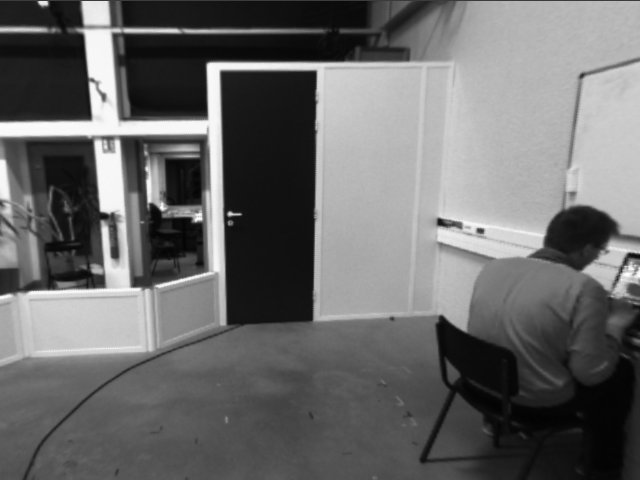
\includegraphics[width=.95\linewidth]{src/chap4-integration/disparity-1.jpg}
    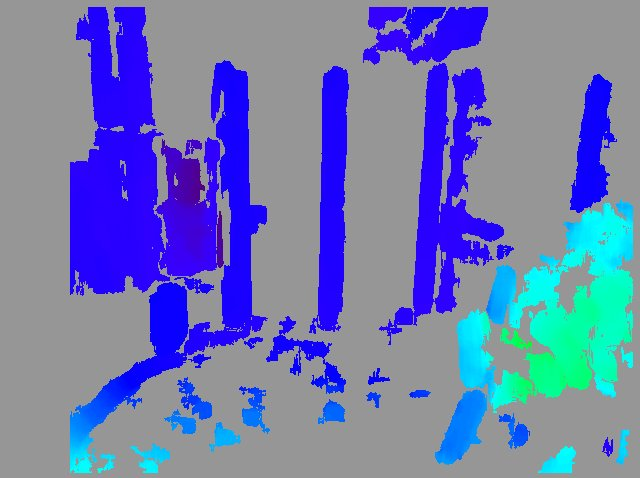
\includegraphics[width=.95\linewidth]{src/chap4-integration/disparity-2.jpg}
  \end{center}
  \caption{Carte de profondeur\index{carte de profondeur} calculée en
    temps réel. Une couleur claire correspond à une faible profondeur,
    une couleur foncée à une profondeur importante. Les zones grises
    indiquent les endroits où aucune correspondance n'a pu être
    établie entre les images de deux caméras. Elles correspondent
    typiquement à une zone peu texturée comme un mur.}
\end{figure}


\begin{figure}
  \begin{center}
    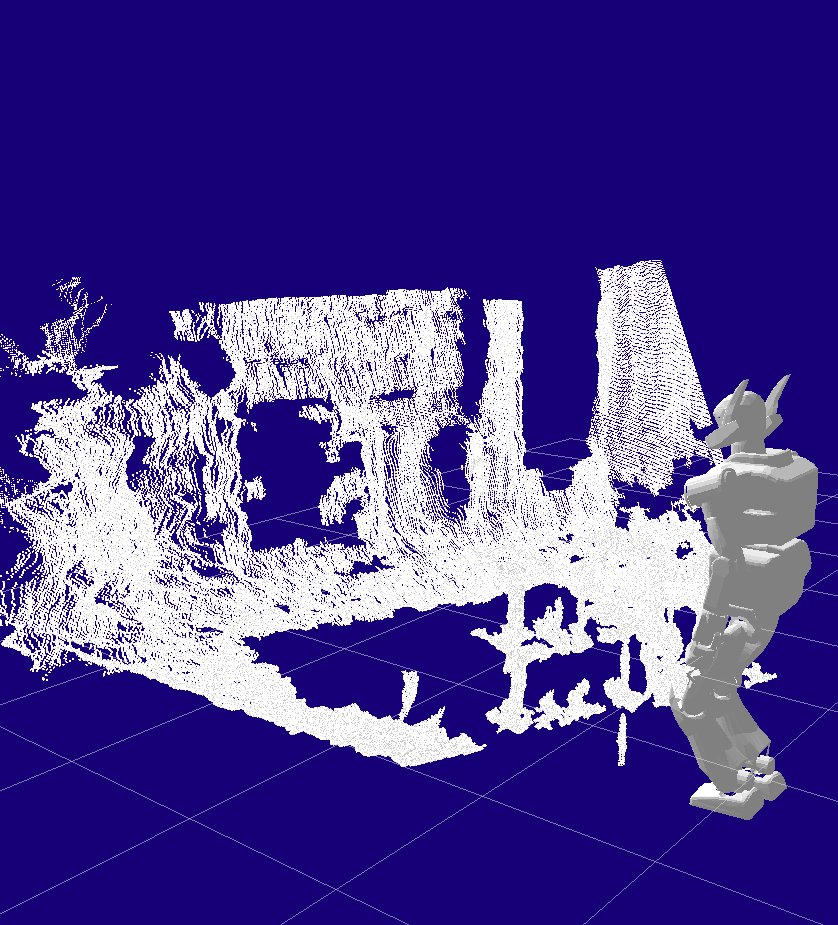
\includegraphics[width=.95\linewidth]{src/chap4-integration/stereo1.jpg}
  \end{center}
  \caption{Reconstruction 3D de l'environnement autour du robot HRP-2
    à partir des données de la paire de caméra stéréo.}
\end{figure}


\subsection{Capture de mouvement}

Une alternative à la vision embarquée est l'utilisation des systèmes
de capture de mouvement. Ces derniers, à l'origine destinés à étudier
les mouvements humains, ont été largement détournés afin de pouvoir
suivre les mouvements d'objets autour du robot et s'abstraire des
difficultés propres à la perception en robotique.


Un composant réalisant l'interface entre d'une part, le système de
capture de mouvement, et l'architecture robotique d'autre part a été
écrit. Ce dernier permet de suivre les mouvements de plusieurs objets
simultanément et publie une estimation de leur pose via le système de
``topics'' précédemment décrit.


\subsection{Diagnostics et sûreté}

L'utilisation d'un robot humanoïde de grande taille présente toujours
un risque, et ce dernier tend à croître quand l'architecture devient
plus complexe et intègre des composants moins fiables. Pour ce faire,
il est donc nécessaire de pouvoir obtenir un état complet du système
de manière unifiée. Ce dernier est disponible sur le robot et est
illustré par la \autoref{fig:diagnostic}. De plus, il est nécessaire à
tout moment de pouvoir avoir un retour si le mouvement exécuté
présente le risque d'endommager le robot. Ces risques se divisent en
différentes catégories:
\begin{description}
\item[Endommagement des capteurs.] Les capteurs de force sont conçus
  pour résister à un impact de 1000N au plus. Il est recommandé de ne
  pas aller au-delà de 800N par mesure de sécurité. Les autres
  capteurs ne présentent pas de risque particulier.
\item[Endommagement des actionneurs.] Les actionneurs peuvent fournir
  un couple maximal. Au-delà de ce dernier, il risque de chauffer de
  manière trop importante et d'être rendu inopérant. On peut donc
  fixer une borne ``raisonnable'' qui ne devrait jamais être
  dépassée. Évidemment, ceci ne représente qu'une approximation très
  simple des capacités maximums des actionneurs. En particulier, un
  retour sur la température des actionneurs se révélerait être un
  indicateur intéressant, mais n'est malheureusement pas disponible en
  l'état actuel des capacités du robot.
\item[Instabilité lors de la locomotion.] Il est possible d'estimer la
  position du ZMP\index{Zero-Momentum Point} à partir des forces
  mesurées par les capteurs de force. Cette estimation permet
  d'avertir l'utilisateur quand le ZMP se rapproche dangereusement de
  la limite du polygone de sustentation.
\item[Déviation des horloges des ordinateurs embarqués.] Les
  ordinateurs embarqués synchronisent leurs horloges en utilisant le
  protocole NTP -- Network Time Protocol --\index{Network Time
    Protocol (NTP)}. L'ordinateur dédié à la décision et la perception
  se synchronisent sur un serveur de temps distant. L'utilisation d'un
  lien WiFi et la présence de routeurs intermédiaires rendent la
  synchronisation relativement peu précise. Cependant, le problème
  n'est pas très gênant, car le véritable enjeu reste de faire en
  sorte que les deux PCs embarqués gardent leurs deux horloges
  synchronisées. Le lien réseau étant direct, la synchronisation
  relative de ces deux ordinateurs est, au contraire, de très bonne
  qualité et permet d'assurer la cohérence des données temporelles
  entre, d'une part, le contrôleur commandant les actionneurs, et
  d'autre part les composants de décision et de perception.
\item[Difficultés informatiques d'ordre général.] Au-delà des problèmes
  décrits précédemment et qui affectent plus particulièrement les
  systèmes robotiques, les robots sont également affectés par
  l'ensemble des problèmes qui peuvent toucher un ordinateur:
  température excessive du processeur, manque d'espace de stockage,
  etc.
\end{description}

Une des difficultés de la mise en \oe uvre d'un système robotique est
la nécessité de faire fonctionner un ensemble de technologies sachant
que le mauvais fonctionnement de n'importe quel morceau de
l'architecture peut mettre en péril la tâche tout entière. Qui plus
est, certaines limitations du matériel tel que le couple maximum des
actionneurs sont parfois vérifiées a posteriori. Des systèmes de
surveillance des valeurs critiques sur les couples, les impacts sur
les capteurs de force ont donc été mis en place afin d'éviter
d'endommager le matériel.


\section{Simulation transparente}


Une difficulté récurrente en robotique est la lenteur de la
réalisation des expérimentations: calibrer un robot et réaliser une
expérience demande beaucoup de temps. Afin d'accélérer au maximum le
développement et d'assurer la sécurité des expérimentateurs et du
matériel, une phase de simulation des expérimentations reste cruciale.


L'utilisation d'une architecture robotique fondée sur un modèle de
communication donne ici tout son intérêt: la totalité des capacités du
matériel, tant au niveau de l'actionnement que des capteurs est
représenté informatiquement par un ensemble composé de services et de
``topics''. Tant que le simulateur choisi fournit ce même ensemble de
canaux de communication, les algorithmes pourront fonctionner
indifféremment en simulation ou sur le véritable système. Il reste
alors le plus important: assurer la cohérence entre les capteurs
simulés en fonction des commandes envoyées aux actionneurs. Pour ce
faire, il est important de disposer d'un moteur physique
réaliste. Dans le cadre de cette thèse, le simulateur
OpenHRP\index{OpenHRP (simulateur dynamique)} a été choisi. En effet,
la plupart des simulateurs robotiques -- Gazebo, Webots --, utilisent
des moteurs physiques primitifs adaptés aux robots mobiles ne
réalisant pas de mouvements ``dynamiques''. Afin de modéliser
précisément les interactions entre le pied et le sol, un moteur
physique disposant d'un modèle de contact convaincant et précis est
indispensable à la simulation d'un mouvement réalisé par un robot
humanoïde.


Les limitations de la plate-forme sont généralement liées à la
simulation des caméras, ne pouvant jamais reproduire les difficultés
inhérentes à la vision par ordinateur: changements d'illumination,
délai induit par l'acquisition et le transfert des données, erreur de
calibration de la caméra, etc. La simulation est donc davantage un
moyen de tester la correction du raisonnement et pas tant un outil
fiable pour démontrer sa robustesse à la réalité qui diverge toujours
du modèle calculé.


\section{Modélisation unifiée d'un système robotique}


La génération de mouvement se fonde sur une connaissance précise des
capacités physiques des robots. Cette description est généralement
codée à l'aide d'un format de fichier permettant de représenter les
différentes informations caractérisant le système. Une définition
mathématique du système a été donnée dans le \autoref{chap:suivi}. Du
point de vue informatique, le format de fichier URDF -- Unified Robot
Description Format --\index{Unified Robot Description Format (URDF)},
SRDF -- Semantic Robot Description Format --\index{Semantic Robot
  Description Format (SRDF)} et RCPDF -- Robot Contact Point
Definition Format --\index{Robot Contact Point Description Format
  (RCPDF)} est utilisé pour représenter les informations nécessaires à
la génération de mouvements sur un robot humanoïde. Les deux premiers
formats sont le fruit du travail de la communauté ROS tandis que le
dernier a été développé dans le cadre de cette thèse.

\begin{figure}
  \begin{center}
    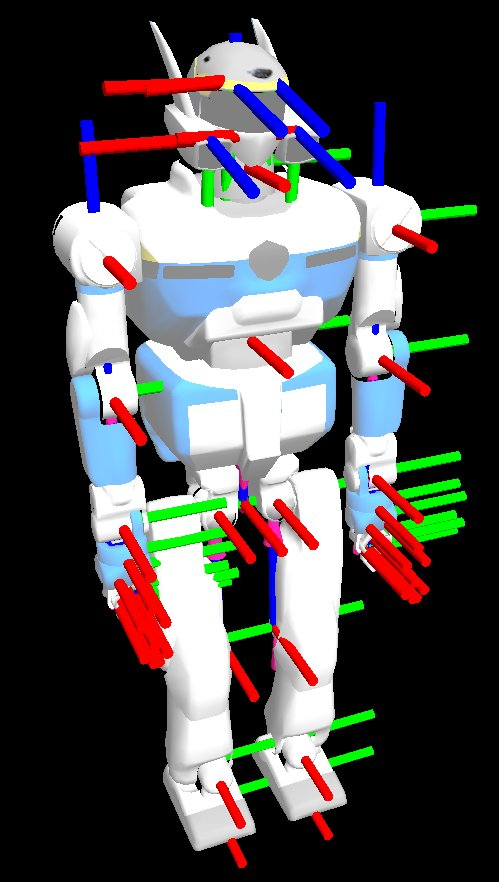
\includegraphics[width=.45\linewidth]{src/chap4-integration/hrp2_urdf.jpg}
  \end{center}
  \caption{Modèle de robot HRP-2 décrit via le format URDF.}
\end{figure}



\subsection{Description d'un robot}


Un robot est un ensemble de corps dont les mouvements relatifs sont
contraints. La modélisation des contraintes passe par la modélisation
des articulations reliant deux corps entre eux. Le format URDF définit
donc deux grands types d'objets: les corps et les articulations. Nous
allons voir quelles informations sont attachées à chaque type d'objet.

\paragraph{Corps}

Un corps est défini par une forme géométrique. Cette forme peut soit
être définie par une primitive géométrique commune -- sphère,
cylindre, boîte -- ou bien via un modèle 3D. Les informations de la
dynamique du corps sont également codées: position du centre de
masse au sein de l'objet ainsi que la matrice d'inertie associée au
corps. Une représentation alternative de la géométrie du corps
utilisée pour les calculs des collisions peut également être
définie. Dans le cas d'HRP-2, une version alternative des modèles des
corps utilisant une approximation convexe avec un pas de dicrétisation
plus grossier est disponible afin de pouvoir accélérer l'évaluation
des collisions. Une version alternative fondée sur l'utilisation de
capsules est également utilisée afin de fournir des tests de collision
rapides pour la planification de mouvements.


\paragraph{Articulation}

Une articulation lie deux corps tout en imposant un ensemble de
contraintes au mouvement relatif de ces deux éléments. Un joint
comporte donc un lien vers le corps ``père'' et le corps ``fils'' pour
définir sa position dans l'arbre cinématique. Dans le cas du joint
racine, il peut ne pas y avoir de corps ``père'' et dans le cas d'un
organe terminal, il peut ne pas y avoir de corps ``fils''.

Les joints supportés sont les suivants:
\begin{description}
\item[Libre.] Ce joint virtuel possède six degrés de liberté et
  n'impose aucune contrainte.
\item[Rotation.] Ce joint possède un degré de liberté unique et impose
  un mouvement de rotation autour d'un axe spécifique au joint.
\item[Translation.] Ce joint possède un degré de liberté unique et
  impose un mouvement de translation le long d'un axe spécifique au
  joint.
\item[Planaire.] Ce joint possède deux degrés de liberté et impose un
  mouvement coplanaire à un plan spécifique au joint.
\item[Fixe.] Ce joint ne possède pas de degré de liberté et impose un
  mouvement rigide entre les deux corps.
\end{description}

Les degrés de liberté des joints possèdent généralement un minimum et
maximum qui sont soit le résultat de la conception mécanique du joint,
soit lié à la géométrie du robot: une valeur différente entraînerait
immédiatement une autocollision et il n'est donc pas intéressant de
considérer ces valeurs. Chaque joint comporte donc ces valeurs ainsi
qu'une vitesse et une force ou un couple maximum selon le type de
joint. Enfin la friction statique du joint ainsi que l'amortissement
utilisé pour la simulation de ce dernier peuvent également être
enregistrés.


\paragraph{Capteurs}

Une fois l'arbre cinématique défini et annoté par les corps du robot
auquel ils sont attachés, il reste encore un élément clé à spécifier:
la position des capteurs. Pour ce faire, des joints fixes définissent
la position de corps ``virtuels'' sans géométrie permettant de
spécifier la position de points importants du robot tels les capteurs.

Il n'y a malheureusement pas de description générique de ces derniers
qui permettrait de ne pas abuser de la structure cinématique du robot.


\subsection{Modélisation des préhenseurs du robot HRP-2}

La complexité du processus de génération de mouvements pour un système
croît avec le nombre de degrés de liberté. Par exemple,
HRP-2\index{HRP-2} est un système possédant 40 degrés de
liberté\index{degré de liberté}, dont 10 pour les mains. Cependant,
tous ces degrés de liberté ne sont pas commandables. En effet, chaque
main n'est commandée que par un seul degré de liberté décrivant le
niveau de fermeture de la pince. Ces mécanismes sont régulièrement
utilisés dans les robots. On peut également citer le robot Romeo
d'Aldebaran Robotics\footnote{Description officielle du prototype de
  plate-forme: \url{http://projetromeo.com/}} qui s'appuie sur un
mécanisme de commande similaire: un degré de liberté commande
l'actionnement d'une main complète composé de plusieurs degrés de
liberté. Pour modéliser un tel système, il est possible d'insérer des
contraintes et des degrés de liberté ``dépendants'' dans le modèle. On
peut ainsi insérer une contrainte qui va lier deux degrés
ensemble. Par exemple dans la définition du joint A, on peut spécifier
que la valeur du degré de liberté associé dépend de la valeur du degré
de liberté du joint B:

\begin{equation}
  \mathbf{X}_B = \alpha_B \mathbf{X}_A + \beta_B
\end{equation}

Dans l'équation précédente, $\alpha_B$ et $\beta_B$ sont des
constantes propres au joint B. $\mathbf{X}_A$ et $\mathbf{X}_B$ la
valeur du degré de liberté associé respectivement aux joints A et B.


\subsection{Prise en charge des autocollisions}

Une autocollision consiste en la collision de deux corps du
robot. C'est particulièrement facile sur un humanoïde: les bras et les
jambes formant quatre chaînes distinctes pouvant entrer en collision
les unes avec les autres. D'autres cas sont également possibles: par
exemple la jambe de certains robots HRP-2 peut entrer en collision
avec le bassin dans certaines configurations. De manière générale,
toute collision qui requiert le mouvement de plusieurs degrés de
liberté combinés et qui ne peut donc pas être évitée en spécifiant les
bornes des degrés de liberté est une autocollision qui doit être prise
en compte.

Pour déterminer les autocollisions, deux stratégies sont
possibles. L'approche automatique consiste à échantillonner l'espace
des configurations du robot afin de trouver les corps qui sont soit
toujours en collision soit jamais en collision. Dans ces deux cas, la
paire de collision est rejetée. Toutes les autres sont ajoutées.  La
seconde stratégie consiste à forger la liste à la main. Dans le cas où
les autocollisions doivent être vérifiées dans la boucle temps réel,
cette technique est souvent utilisée, car les contraintes de temps de
calcul sont trop fortes pour considérer toutes les paires. On se
concentre alors sur les cas les plus probables. En particulier,
certains cas semblent difficiles à détecter automatiquement, notamment
si pour entrer en collision avec le corps A, il faut forcément
traverser le corps B alors il est inutile de prendre en compte le
corps A lors de la vérification des autocollisions.

La liste des paires de collisions est enregistrée dans un fichier
séparé utilisant le format SRDF -- Semantics Robot Description Format
--\index{Semantic Robot Description Format (SRDF)}. Ce fichier stocke
également la position de référence du robot dans lequel il se situe
lors du démarrage des expérimentations.


\subsection{Définition des contacts autorisés}

Un défi ouvert pour la robotique humanoïde dans les prochaines années
est la réalisation de mouvements asservis sur des sols non plans ou
utilisant des contacts avec d'autres zones du corps que les
pieds. Pour un robot donné, les contacts sont autorisés à différents
endroits, typiquement, les mains et les pieds. Il est donc nécessaire
de définir des ``zones'' où les contacts sont autorisés. Cette
information n'était pas formalisée jusqu'à présent dans l'architecture
proposée par ROS et a été le résultat d'un travail réalisé durant
cette thèse. Le format de fichier RCPDF -- Robots Contact Point
Description Format --\index{Robot Contact Point Description Format
  (RCPDF)} associe à chaque corps 0, 1 ou plusieurs zones de
contact. Chaque zone de contact peut être soit représentée par une
primitive géométrique soit par un modèle 3D. Les normales du modèles
permettent de définir la direction dans laquelle le contact peut
s'effectuer. Un contact est valide si la force de réaction de
l'environnement sur le corps du robot est colinéaire avec la normale
de la zone de contact mais de direction opposée. Enfin, la force de
réaction maximale en un point autorisée sur cette zone de contact peut
être enregistrée afin d'assurer que le contact ne va pas compromettre
l'intégrité structurelle du robot. Cette représentation offre une
formulation générique qui peut être utilisée pour réaliser des prises
de décisions moins arbitraires que celles qui sont uniquement fondées
sur l'anthropomorphisme. Par exemple, la force applicable sur les
mains du robot peut être plus contrainte ce qui peut pousser un
solveur à faire marcher le robot ``sur ses deux jambes'' sans avoir à
le lui spécifier de manière directe.

En pratique, ces données sont utilisées dans les algorithmes de marche
bipèdes et les systèmes de surveillance afin de calculer les tailles
des semelles du robot -- la zone de contact autorisée sous chaque pied
-- et, de fait, les contraintes auxquelles sont soumises le ZMP.


\subsection{Adaptation du modèle pour le contrôle et la planification}

Instrumenter le modèle pour y incorporer le maximum d'informations est
intéressant, cependant utiliser la chaîne cinématique pour positionner
des capteurs pose des problèmes pratiques. En effet, l'évaluation de
l'arbre est nécessaire pour de nombreux calculs qu'ils soient
géométriques, cinématiques ou dynamiques, inverses ou directs. La
complexité de ces algorithmes est donc dépendante de la taille de
l'arbre et la présence d'articulations, même fixes, pour positionner
les capteurs crée un coût supplémentaire qui semble inutile. Une
proposition est en cours pour modéliser d'une manière plus propre les
capteurs dans le format URDF, mais à l'heure actuelle il semble
intéressant de pouvoir réaliser des simplifications ou ``élagages'' de
l'arbre pour pouvoir en retirer les éléments qui ne sont pas
nécessaires. Dans le cas où les corps que l'on souhaite supprimer sont
des n\oe uds terminaux de l'arbre sans information dynamique -- comme
les capteurs --, alors l'opération peut être réalisée
directement. Cependant, dans tous les autres cas, il est nécessaire de
pouvoir calculer la masse et l'inertie équivalente de l'ensemble des
corps rendus solidaires par la simplification opérée. De fait, ces
transformations de l'arbre sont un moyen bien plus efficace d'exprimer
les contraintes égalités sur certains degrés de liberté que leur
insertion en tant que contrainte dans l'algorithme de génération de
mouvement proprement dit. Les transformations dynamiques de l'arbre
sont également nécessaires pour adapter la géométrie du robot
lorsqu'il est nécessaire, par exemple, de réaliser une tâche de
locomotion en transportant un objet possédant un poids non négligeable
pouvant interférer dans la dynamique du mouvement.

Le système de représentation du robot peut d'ores et déjà coder la
totalité des informations proposées dans cette section, mais il n'a
pas été possible, à l'heure actuelle, d'intégrer le mécanisme de
transformation de l'arbre aux logiciels de planification et de
contrôle utilisés sur le robot humanoïde HRP-2.


\section{Applications robotiques}


L'ensemble des outils décrits dans la section précédente doit être
mis en \oe uvre conjointement afin de pouvoir former une architecture
robotique cohérente. Chaque composant faisant partie d'une
architecture robotique a beau disposer d'un modèle de communication
cohérent, sembler parfaitement fonctionner pris à part et malgré tout
l'assemblage du tout reste une opération délicate: a-t-on suffisamment
de ressources pour faire fonctionner tous les composants à une vitesse
raisonnable? A-t-on une bande passante suffisamment importante entre
les ordinateurs pour communiquer les informations transmises? Le délai
de transmission perturbe-t-il l'architecture? La totalité de ces
questions ajoutées aux difficultés inhérentes au déploiement d'une
application logicielle distribuée nécessite une grande rigueur dans le
développement des démonstrations. Nous allons ici développer un
exemple de scénarii puis montrer quel bilan on peut tirer des séries
d'expériences réalisées durant cette thèse.


\subsection{Mise en place d'une application}


Nous allons présenter dans cette section l'architecture de la
démonstration robotique présentée dans la
\autoref{sec:chap3_localisation}: le robot HRP-2 doit pouvoir réaliser
une tâche de locomotion pour se déplacer jusqu'à un meuble dans lequel
il souhaite déposer un objet -- dans cet exemple une balle rose
--. Pour ce faire, il doit tout d'abord planifier une trajectoire
corps complet, c'est-à-dire combinant à la fois locomotion et
manipulation. Une fois cette trajectoire déterminée, il doit
l'exécuter tout en corrigeant sa trajectoire afin d'atteindre son
but. La localisation est réalisée grâce aux caméras du robot.

Le système est composé des composants robotiques suivant répartis sur
deux ordinateurs -- un pour le contrôle et l'autre pour la décision et
la perception --:
\begin{description}
\item[Ordinateur dédié au contrôle.]
   \\
  \begin{description}
  \item[Contrôle.] Ce n\oe ud est composé d'un solveur fondé sur le
    paradigme de la pile de tâches et d'une infrastructure logicielle
    utlisant le langage de programmation Python pour insérer et
    définir des tâches en cours d'exécution. Les références des tâches
    peuvent être fournies par l'extérieur via des topics. Ce composant
    fonctionne partiellement en temps réel.
  \item[Export des informations capteurs et de la
    commande\footnote{Composant remplacé lors de la simulation par un
      n\oe ud fournissant les mêmes services dans le monde
      simulé.}\addtocounter{footnote}{-1}\addtocounter{Hfootnote}{-1}.]
    La commande envoyée au système, la commande après stabilisation et
    l'état actuel du robot lu sur les encodeurs est publié sous la
    forme de topics. L'accélération linéaire et la vitesse angulaire
    du torse du robot sont également publiés sous la forme d'un
    topic. Ce composant fonctionne partiellement en temps réel.
  \end{description}

\item[Ordinateur dédié à la décision et à la perception.]
   \\
  \begin{description}
  \item[Acquisition des images.\footnotemark] Capture les images venant de la paire
    stéréo grand angle.
  \item[Conversion de l'espace couleur.] Transforme les images encodées
    en Bayer vers des images monochromatiques.
  \item[Rectification.] Corrige la déformation de l'image liée à
    l'utilisation de l'objectif grand angle et à la conception de la
    caméra.
  \item[Localisation.] Réalise une estimation de la position du robot
    dans le monde en utilisant les caméras du robot.
  \item[Cinématique directe.] À partir de l'état des encodeurs, ce
    composant recalcule la position relative de tous les corps et les
    publie sous forme de topics.
  \item[Évaluation de l'erreur de positionnement.] Compare la position
    voulue du robot dans le plan à un instant $t$ à la position perçue
    au même instant.
  \item[Divers.] Plusieurs n\oe uds supplémentaires sont chargés de la
    surveillance des paramètres critiques du robot.
  \end{description}
\end{description}


\begin{sidewaysfigure}[htbp]
  \begin{center}
    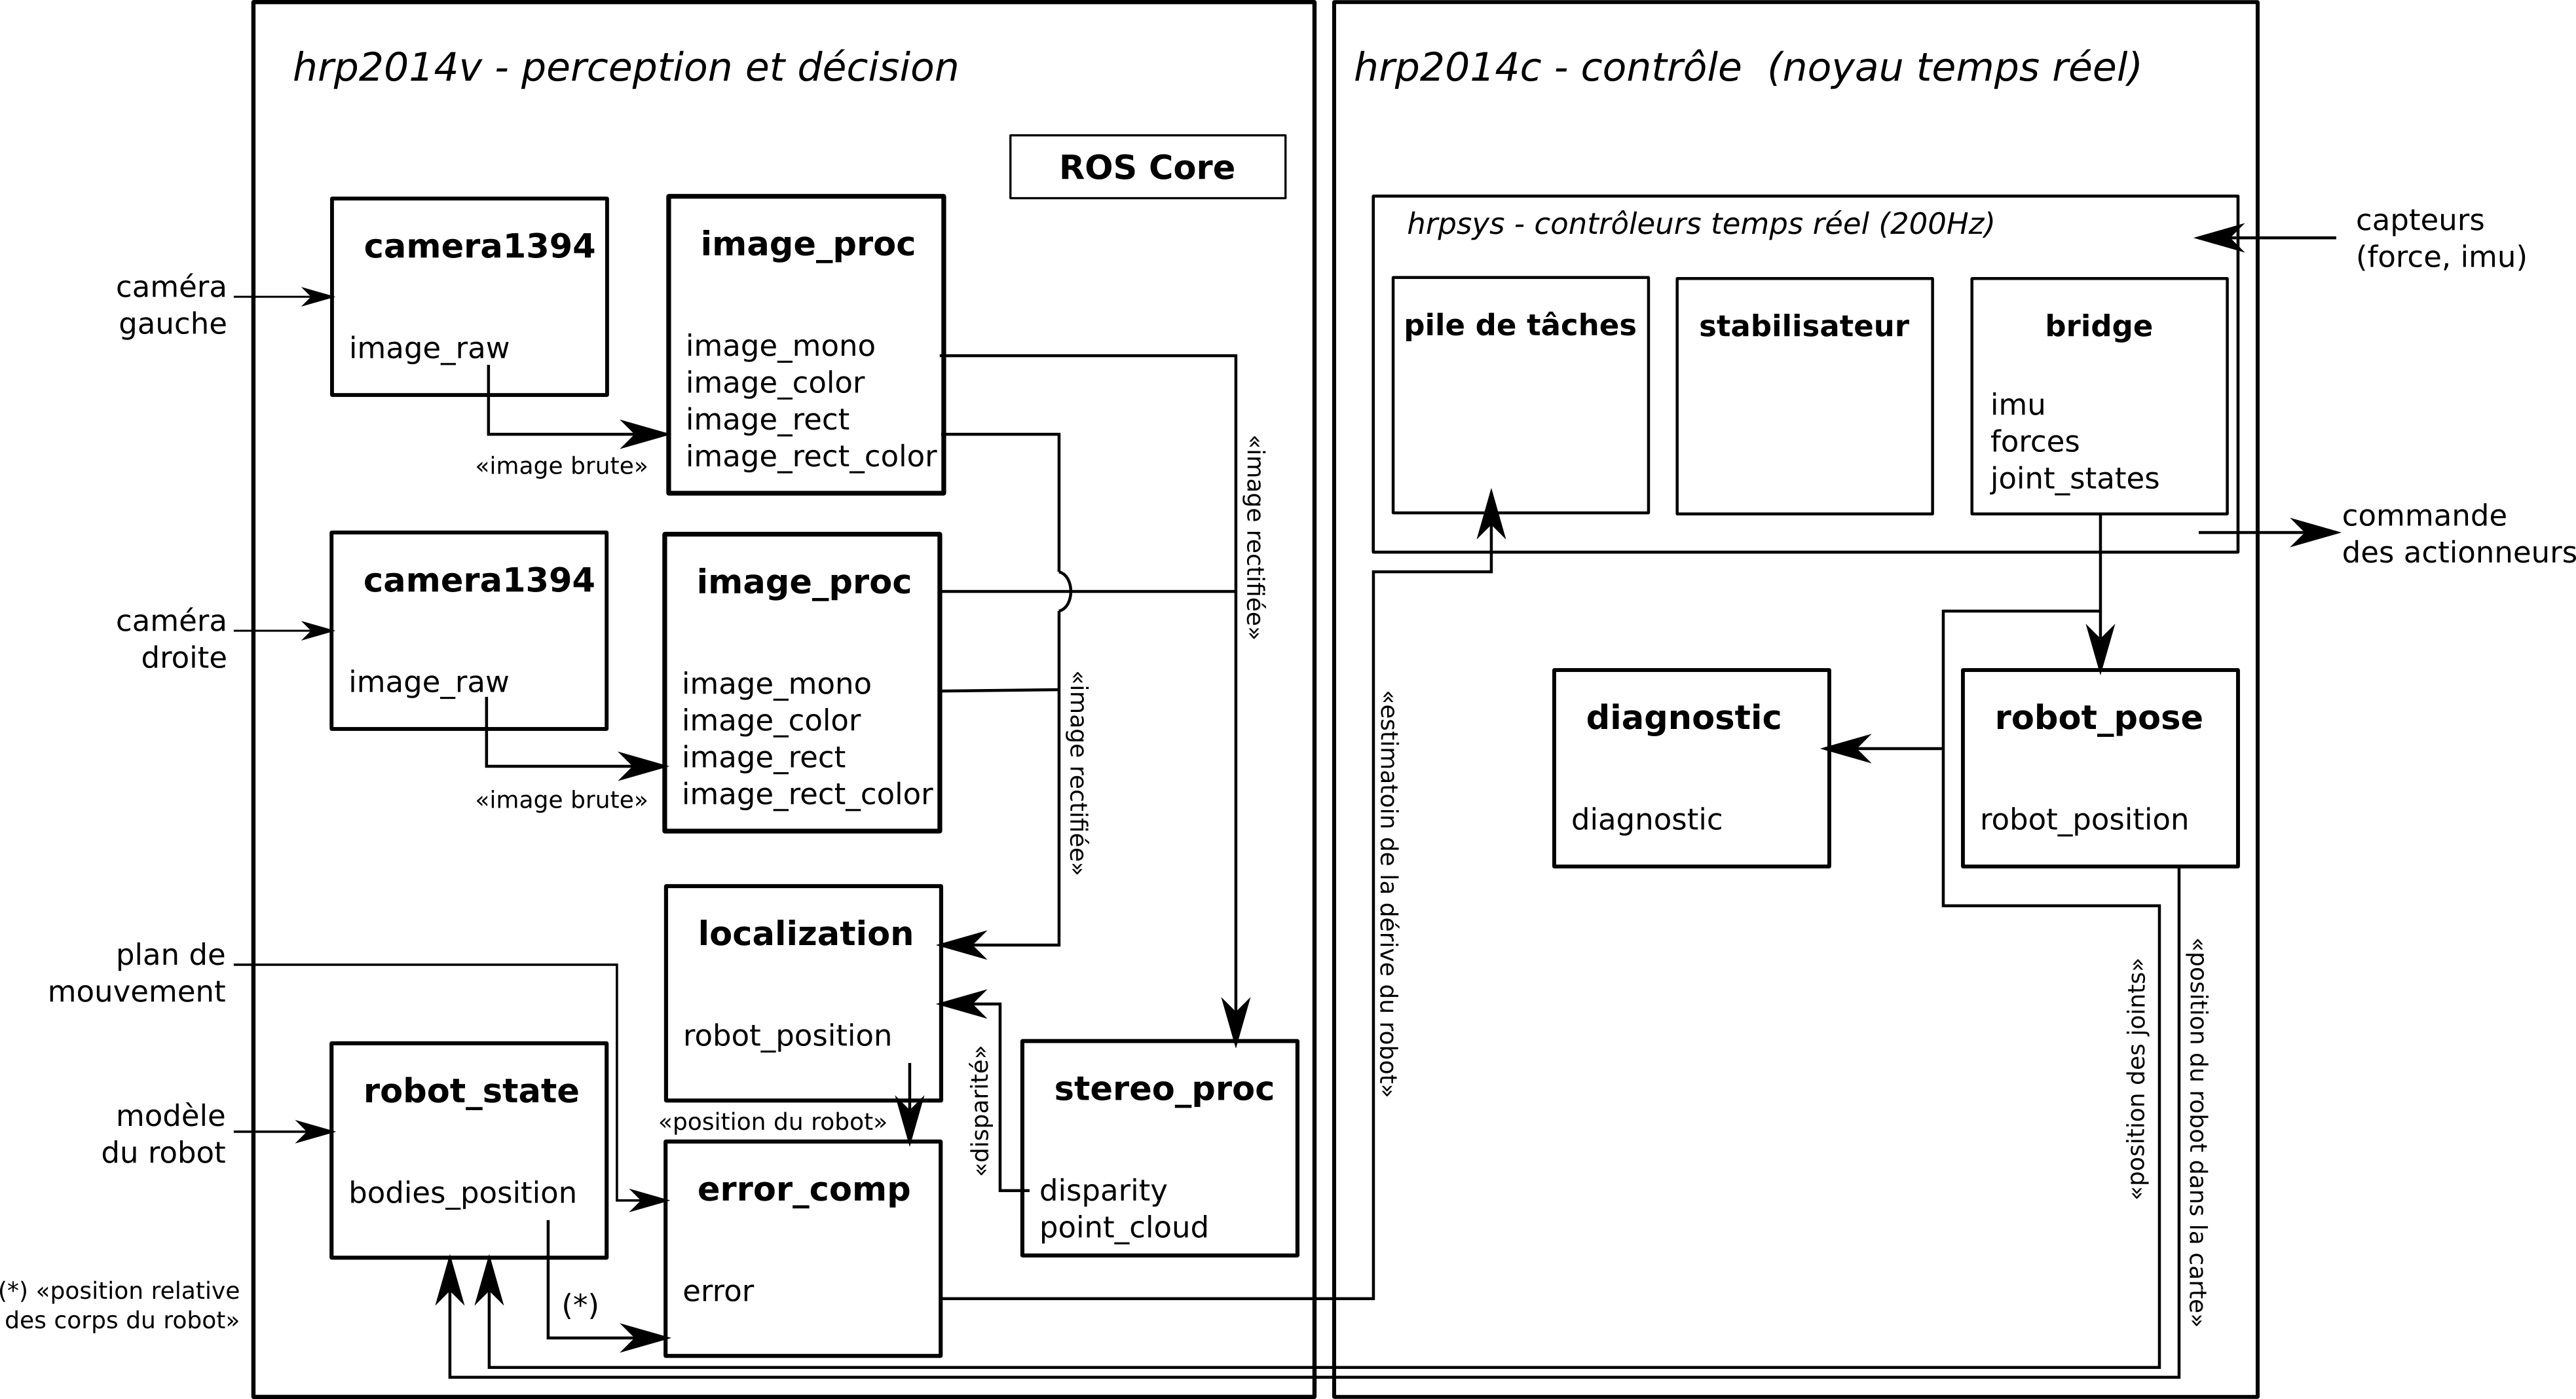
\includegraphics[width=.95\linewidth]{src/chap4-integration/archi.png}
  \end{center}
  \caption{Schéma de fonctionnement de
      l'architecture.\label{fig:roscomponents}}
\end{sidewaysfigure}



Ces composants interagissent entre eux et fournissent chacun des flux
de données et des services qui sont détaillés dans la
\autoref{fig:roscomponents}.


Cette architecture a été testée sur le robot humanoïde
HRP-2\index{HRP-2}. L'architecture a fonctionné correctement, mais il
n'a pas été possible d'atteindre une précision suffisante au sein du
système de perception pour compenser avec succès la dérive du
robot. En effet, le SLAM\index{Simultaneous Localization and Mapping
  (SLAM)} tel que configuré ici a donné une précision de plus ou moins
5cm ce qui est insuffisant pour des tâches de locomotions
complexes. On notera également que la phase de planification
n'apparaît pas, elle a été réalisée grâce au travail décrit dans
\cite{11dalibard.humanoids} sous la forme d'un traitement hors
ligne. Le chemin est enregistré sous la forme d'un fichier chargé au
début de l'expérimentation.


\subsection{Difficultés récurrentes}

La mise en place d'une architecture modulaire pour la robotique sert
un objectif principal: contenir la complexité en assurant à
l'utilisateur la possibilité de pouvoir s'abstraire d'une partie des
traitements sous-jacents, quitte à obtenir une solution
sous-optimale. En effet, l'agrégation d'outils aussi différents que la
planification de mouvement, le contrôle, l'asservissement et
différentes techniques de perception nécessite de pouvoir s'appuyer
sur des composants aussi automatiques que possible. En particulier,
concevoir des algorithmes ne nécessitant pas de paramétrage poussé est
important, mais également très difficile. Le paramétrage peut passer
soit par une phase de calibration -- comme souvent en perception --,
une phase de construction de carte, par exemple pour la navigation --
ou le réglage des stratégies adoptées par les algorithmes. Les outils
de planification nécessitent souvent le réglage de paramètres ce qui
complexifie leur utilisation. Si l'on ne peut paramétrer le système
automatiquement, il faut alors tenter de trouver un ensemble de
paramètres ayant une réalité physique qui puisse permettre à
l'utilisateur de se construire plus facilement un modèle de
comportement de l'algorithme.


Une seconde difficulté concerne l'interprétation des données. La
majorité des algorithmes produisent en sortie des données numériques
possédant un sens physique. Prenons par exemple un composant réalisant
le suivi d'un objet en temps réel: il va alors fournir en sortie la
position de l'objet dans l'espace euclidien 3D. Une ambiguïté se pose
alors: par rapport à quel repère référence cette donnée est-elle
exprimée? La caméra du robot? La racine de sa chaîne cinématique? Un
point fixe du monde? Face aux nombreux dysfonctionnements provoqués
par ce type de problème, ROS\index{ROS} fournit une solution clé en
main: chaque transformation précise, sous forme de chaîne de
caractère, de quel repère à quel repère cette donnée est la
transformation. En enregistrant ces données, on acquiert également la
possibilité de calculer automatiquement des transformations d'un
repère à un autre. Par exemple si l'on fournit la transformation de
$A$ à $B$ et de $B$ à $C$, on peut demander la transformation de $A$ à
$C$ et elle peut être calculée automatiquement. Il y a là un véritable
gain puisque l'on passe d'une implémentation dépendant directement des
données des composants auquel on est lié vers une requête purement
sémantique: ``quelle est la position relative de la cheville gauche
par rapport au poignet droit?''. En réalisant une résolution
automatique des transformations, on se préserve également dans le cas
où les composants utilisés changeraient leur repère de référence entre
deux versions. Une fois de plus, l'absence de typage ici rend le
diagnostic difficile: aucune erreur de compilation n'est possible et
les erreurs dans les valeurs numériques elles-mêmes sont toujours
difficiles à détecter. On notera que le système adopté ici se fonde
sur le traitement des chaînes de caractères ce qui est plus lent que le
recours au typage direct tel que proposé dans \cite{12delaet.ram}.


Une troisième difficulté est la robustesse aux phases
transitoires. Tout système complexe possède une phase d'initialisation
dans laquelle le comportement des modules peut être sous-optimal. En
particulier quand plusieurs composants communiquant ensemble sont
lancés en même temps, il n'y a aucune garantie que le premier
composant terminant son initialisation soit toujours le même. De ce
fait, un composant peut commencer à attendre des données sur un topic
avant que le topic ne soit créé par le premier composant. Le protocole
de communication est extrêmement souple sur ce point et la possibilité
de pouvoir écouter des flux de données qui n'existent pas encore
simplifie de beaucoup le développement en évitant les erreurs lorsque
l'ordre d'initialisation change. Par contre, il est alors nécessaire
de mettre en place, en interne, les mécanismes afin d'éviter les
situations de famine où plusieurs composants s'attendent les uns les
autres indéfiniment. Cependant, le graphe de communication étant le
plus souvent un arbre, ce genre de cas reste peu courant.


La quatrième difficulté concerne l'initialisation du système. Il est
souvent difficile de lancer une démonstration en ``un clic'', mais
plus le nombre d'étapes pour démarrer la démonstration est important,
plus le risque d'introduire une erreur humaine lors d'une
expérimentation augmente. Il est important de limiter les opérations
pour démarrer une démonstration. Un outil utilisé dans le cadre de ce
travail est un formalisme permettant de décrire informatiquement -- en
XML\index{XML} --, le graphe formé par l'ensemble des composants
robotiques ainsi que leurs paramètres respectifs. Ce système réduit
donc au maximum les erreurs humaines, mais certaines difficultés
persistent: un robot humanoïde utilisant une commande à gains forts
telle que HRP-2 s'initialise en l'air, puis il doit être posé, le
système possède donc plusieurs phases transitoires d'initialisation
qu'il est difficile d'automatiser.


\begin{figure}[htbp]
  \begin{center}
    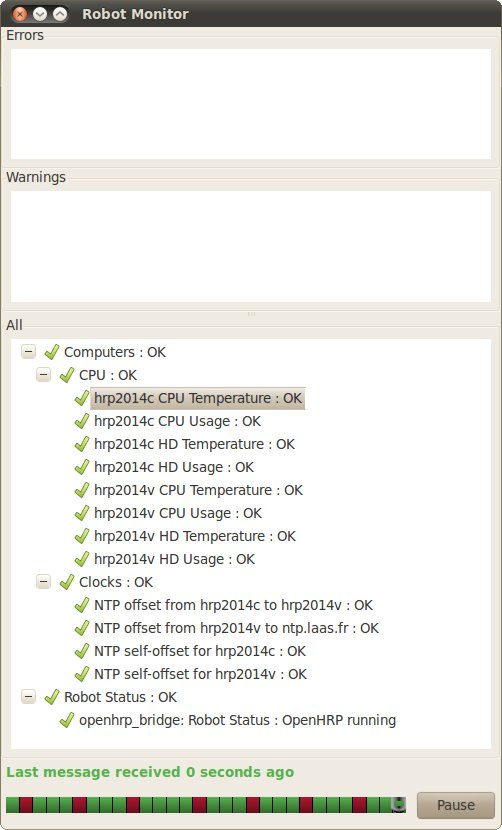
\includegraphics[width=.3\linewidth]{src/chap4-integration/hrp2_diagnostics.jpg}
  \end{center}
  \caption{Visualisation de l'état général du robot fourni par les
    outils de diagnostic automatique.\label{fig:diagnostic}}
\end{figure}



Le dernier problème récurrent est la difficulté pour un utilisateur de
déterminer si le système est dans un état stable et, si ce n'est pas le
cas, arriver à diagnostiquer le système. La section précédente a
développé un ensemble d'outils permettant de surveiller l'état du
robot tant au niveau mécanique, informatique que de l'utilisation qui
en est faite en temps réel -- vérification des couples au niveau des
actionneurs notamment --. Cependant, les problèmes ne viennent pas que
de ces composants ``bas-niveau''. Des composants algorithmiques
peuvent également échouer pour diverses raisons. Pour aider la
compréhension de l'état du système, le premier élément est d'unifier
les mécanismes de rapport d'état. En effet, la plupart des
bibliothèques complexes viennent avec leur système de journalisation
qui n'est pas toujours adapté. Dans le cadre de cette architecture,
nous avons la possibilité de pouvoir agréger les informations dans un
seul topic qui peut ensuite être observé pour connaître l'évolution du
système. On a alors la liste des messages envoyés par les différents
composants dans l'ordre chronologique ce qui n'est pas le cas quand
chacun fonctionne de manière séparée. Les causes et les conséquences
sont, dans ce contexte, bien plus faciles à identifier. Le deuxième
niveau consiste à publier sur le topic de diagnostic l'état du n\oe
ud. Cela correspond à l'un des états suivants: OK, erreur,
avertissement auxquels on associe des données techniques pour aider au
diagnostic, voir \autoref{fig:diagnostic}. Enfin, un service
standardisé peut également être fourni par un composant pour qu'il
tente un autodiagnostic. Ces mécanismes permettent d'aider à la
compréhension des erreurs.



\subsection{Bonnes pratiques pour la robotique}

Cette section détaille la méthodologie à suivre tant pour développer
un composant robotique que pour développer une architecture robotique
complète. Pour développer un composant, un exemple de développement
réalisé pendant cette thèse a été choisi: il s'agit de l'intégration
d'un logiciel de suivi. Le cycle de développement\index{cycle de
  développement} d'une architecture robotique est ensuite détaillé.


\subsubsection{Étude de cas: intégration d'un algorithme de suivi}

Le composant dont il est question ici est librement disponible sur
internet. Il s'agit de la stack ROS\index{ROS}
\texttt{vision\_visp}\footnote{Site officiel:
  \url{http://www.ros.org/wiki/vision_visp}} et plus particulièrement
du paquet \texttt{visp\_tracker}\footnote{Site officiel:
  \url{http://www.ros.org/wiki/visp_tracker}}.


L'algorithme de suivi d'objet a été développé au sein de l'équipe
LAGADIC\footnote{Site de l'équipe LAGADIC:
  \url{http://www.irisa.fr/lagadic/}} -- INRIA Rennes-Bretagne
Atlantique et à l'IRISA--. Cet algorithme utilise l'asservissement
visuel pour calculer une estimation de la pose d'un objet. Le modèle
de l'objet est connu et une estimation initiale de la position de ce
dernier est nécessaire. Une fois cette estimation connue, l'algorithme
tente de minimiser l'écart entre la position des lignes -- bords -- de
l'objet dans l'image par rapport à la reprojection du modèle de
l'objet suivi dans l'image. D'autres critères que les lignes peuvent
être choisis, mais c'est ce dernier point qui a été retenu dans nos
tests. La résolution de ce problème passe par la méthode de
Levenberg-Marquardt\index{Levenberg-Marquardt} qui est proche de
l'algorithme des moindres carrés classiques.


Cet algorithme est partie intégrante de ViSP -- Visual Servoing
Platform -- \footnote{Site du logiciel ViSP:
  \url{http://www.irisa.fr/lagadic/visp/visp.html}}. ViSP intègre
directement des outils pour acquérir des images à partir de caméras ou
lire des données préenregistrées, mais n'est pas un composant
robotique en lui-même.


La première étape a été de concevoir l'interface du composant: flux de données
et services. L'information calculée par ce programme est simple à
définir: il s'agit de la position relative de l'objet suivi par
rapport à la caméra. On peut donc ajouter un repère supplémentaire à
l'annuaire de transformations afin de spécifier la position de l'objet
suivi. Il sera dès lors possible de calculer, par exemple, la position
relative du poignet par rapport à cet objet pour tenter de
l'atteindre, s'il existe une chaîne entre de transformations entre ces
deux repères. En entrée, le problème est plus complexe. Il faut d'une
part un flux d'images, des informations de calibration, un modèle 3D de
l'objet à suivre et un jeu de paramètres permettant de régler
l'algorithme de suivi ainsi qu'une pose initiale.

\begin{figure}
  \begin{center}
    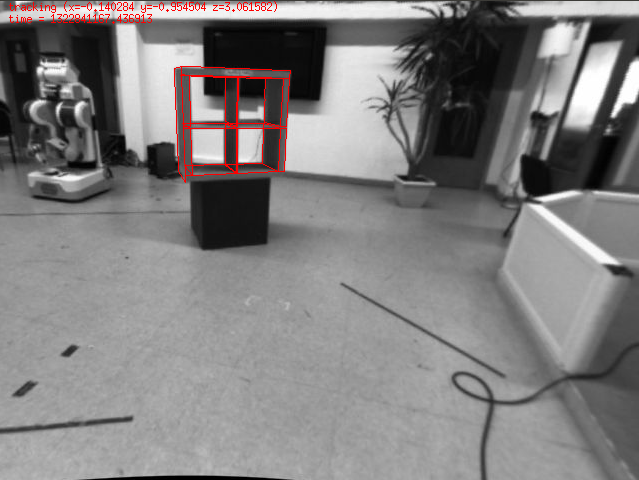
\includegraphics[width=.95\linewidth]{src/chap4-integration/shelf.png}
  \end{center}
  \caption{Le visualisateur associé au composant de suivi d'objet.}
\end{figure}



Il est courant de modéliser le comportement des composants robotiques
sous la forme d'une machine à état. Dans notre cas le composant de
suivi est dans un état ``non initialisé'' au départ où il reçoit déjà
des images et des informations de calibration, mais ne réalise aucun
traitement. Un service permet d'initialiser le suivi en fournissant à
la fois la pose initiale de l'objet, son modèle et les paramètres de
suivi. Le n\oe ud passse alors dans un état actif où il réalise le
suivi. Si le suivi est perdu à un moment ou un autre, le n\oe ud passe
dans un état ``perdu'' où il tente de réinitialiser le suivi avec la
dernière position connue. Si une estimation de la position de la
caméra est disponible, elle va être utilisée pour tenter de fournir
une estimation de la nouvelle position de l'objet en considérant ce
dernier statique. À n'importe quel moment le service d'initialisation
permet de relancer le suivi.


Afin de simplifier l'utilisation du n\oe ud, deux programmes
additionnels sont fournis: le premier permet de calculer une pose
initiale de manière graphique. L'utilisateur peut cliquer sur des
points de l'objet prédéfini et dont on connaît la position relative en
trois dimensions dans l'objet. Cet outil transmet également au
composant de suivi le modèle de l'objet. Le contexte distribué de
l'application empêche de passer directement des emplacements de
fichiers, car il n'y a aucune garantie que le composant réalisant le
suivi et le programme réalisant l'initialisation partage leur système
de fichier. Le modèle est donc directement transmis sous sa
représentation textuelle via le réseau. De plus, le composant pouvant
être lancé à distance, laisser l'utilisateur spécifier le chemin vers
le modèle sous la forme d'un chemin local est une mauvaise idée, car
il sera tenté d'y insérer le chemin sur sa machine et non sur celle où
le composant va être lancé. Pour ce faire, l'emplacement du modèle est
passé sous la forme d'une URI -- Uniform Resource Identifier
-- \citep{rfc2396}.


Le second outil permet de surveiller l'état du tracking en affichant
non seulement la reprojection du modèle dans l'image, mais surtout
l'état du suivi des lignes du modèle. L'algorithme pouvant rejeter des
points pour différentes raisons, cet outil fournit un retour graphique
de ces informations afin d'aider l'utilisateur à trouver le meilleur
ensemble de paramètres pour optimiser le suivi.


Le dernier point à considérer a été d'intégrer le modèle de
calibration de ROS\index{ROS} à ViSP. En effet, ROS annote chaque
image avec les paramètres intrinsèques de caméra\index{paramètres
  intrinsèques (d'une caméra)}. Ces données sont exprimées sous forme
matricielle et doivent être converties avant d'être mises à jour dans
ViSP ce qui nécessite un traitement simple. L'avantage étant que de
cette manière, on peut complètement contourner le processus de
rectification de ViSP qui nécessiterait une calibration spécifique
pour l'utilisation de ce composant.


Les difficultés rencontrées durant cette intégration sont nombreuses:
il a fallu supprimer le code interactif, notamment pour calculer la
pose initiale qui nécessite de cliquer sur une image. Un tel code ne
peut pas fonctionner sur le robot. Il a fallu s'abstraire du système
de fichier local afin de rendre le système facilement distribuable et
il a fallu trouver une façon de pouvoir exprimer les informations de
``debug'' de manière minimale. Une solution aurait été de tracer une
image avec le résultat du suivi, mais les robots étant souvent reliés
en WiFi à la console le contrôlant, transmettre un tel flot
d'information n'est pas justifiable. À la place, un topic
supplémentaire pour les développeur a été ajouté. Le défi est alors
d'assurer la cohérence des données entre d'un côté les images
provenant du composant de vision, de la pose provenant du tracker
ainsi que du topic transportant les informations supplémentaires pour
les développeurs. Ces informations sont filtrées afin que seul les
triplets présentant un temps identique soient affichés. En effet, dans
les précédentes versions, cette synchronisation n'était pas
réalisée. On avait alors l'impression que le suivi était de mauvaise
qualité alors que le problème venait simplement de l'affichage. Les
paramètres de tracking sont également modifiables durant l'exécution
afin de simplifier la recherche du meilleur paramétrage. Cela ouvre
également la possibilité pour un composant de plus haut niveau, de
changer le comportement du logiciel de suivi et réaliser de ce fait,
une forme de suivi ``supervisé''. On notera qu'une fois de plus, la
définition des paramètres joue un rôle très important. Ici l'absence
de sens physique de certains d'entre eux est dommageable: par exemple
la recherche de la nouvelle pose se fait dans un voisinage qui est
défini en pixel. En pratique, cela signifie que si l'on se rapproche
de l'objet, l'absence de reconfiguration de ce paramètre va causer
l'échec du suivi. Un meilleur paramètre aurait été de passer par une
borne sur la vitesse maximum de la caméra qui aurait permis d'avoir un
comportement cohérent quelque soit la distance à l'objet.


Au final, ce composant a reçu un accueil favorable de la communauté
avec plusieurs utilisateurs confirmés dans des laboratoires et
sociétés tiers. Ces utilisateurs n'avaient pas d'expérience avec les
techniques d'asservissement visuel avant de tenter d'intégrer ce
composant et ont réussi à obtenir des résultats satisfaisants dans le
cadre de leur utilisation sur des robots différents, notamment le robot
REEM de Pal Robotics\footnote{Site officiel:
  \url{http://www.pal-robotics.com/}}. De ce fait l'objectif qui
consistait à pouvoir maîtriser la complexité de la mise en place d'un
tel mécanisme a été rempli au travers des choix réalisés ici. Ce
composant a pu être utilisé dans le cadre d'une architecture robotique
distribuée sur deux ordinateurs et l'introduction d'une interface au
niveau de la componentisation robotique a permis au robot HRP-2 de se
localiser soit en utilisant ce composant, soit en utilisant un
composant de localisation utilisant des amers visuels, soit encore
le système de capture de mouvement de manière transparente. Seul le
lancement du graphe diffère dans ces trois cas.


\subsubsection{Cycle de développement d'une architecture}


La section précédente a décrit le développement d'un composant en
particulier, mais concevoir une architecture ne revient pas à
simplement dupliquer cette approche autant de fois qu'il y a de
composants nécessaires. Il faut tout d'abord découper le problème en
composants cohérents, puis assigner ces composants à un ordinateur
parmi ceux qui équipent le robot et enfin paramétrer chacun des
composants de manière optimale. Dans la mesure où une approche
modulaire a pour intérêt principal la réutilisabilité des composants,
on sera donc contraint par l'interface des composants préexistants que
l'on devra réutiliser, ainsi que par les contraintes matérielles de la
plate-forme: les caméras d'HRP-2 sont connectées à un PC donné donc le
composant d'acquisition des images ne peut fonctionner que sur ce
dernier. Inversement, les commandes sont envoyées via une carte
connectée au second PC, le composant de contrôle ne pourra tourner que
sur celui-ci. De plus, le temps réel contraint le contrôleur a n'être
constitué que d'un seul processus. Le dernier élément à prendre en
compte est la communication intra-n\oe uds: les communications par
``topics'' ou service induisent un retard qui doit pouvoir être
accepté ou géré convenablement. Un autre élément à prendre en compte
est la bande-passante disponible entre les ordinateurs qui constituent
le robot. Il faut s'efforcer de minimiser la bande passante consommée
entre les ordinateurs. Pour les composants effectuant de l'affichage
ou de la surveillance distant le problème est souvent encore plus
critique dans la mesure où le robot est la plupart du temps connecté
en wi-fi et dispose donc d'un lien avec une bande-passante extrêmement
limitée vers l'extérieur. Cela va donc contraindre les
composants de perception, la plupart du temps gros producteurs et
consommateurs de donnée, à se situer sur le même hôte. Une fois le
traitement des images terminé, le résultat final peut représenter un
volume d'informations bien plus compact: trajectoire ou position 3D par
exemple.


En considérant la répartition des composants sur les différentes
machines, il faut déterminer la liste des composants nécessaires. En
général, on part d'un côté de la liste des capteurs que l'on souhaite
utiliser, que l'on fait communiquer avec les algorithmes utilisant ces
données en entrée qui eux-mêmes communiquent avec la partie
décisionnelle. Cette partie étant généralement algorithmique, le
positionnement de ces composants n'est pas soumis à des contraintes
techniques fortes. Enfin, un composant de contrôle est nécessaire pour
envoyer les commandes.


Une fois les n\oe uds choisis et paramétrés, l'étape suivante est la
simulation. De nombreux outils permettent de simuler un mouvement
dynamique dans un monde virtuel. Il est nécessaire ici de remplacer
les composants réalisant l'acquisition des données capteurs par des
composants accédants aux informations équivalentes simulées et le
contrôleur par un contrôleur envoyant sa commande au simulateur. Une
phase supplémentaire de définition du monde est souvent nécessaire.


%\begin{figure}[htbp]
%  \begin{center}
%    %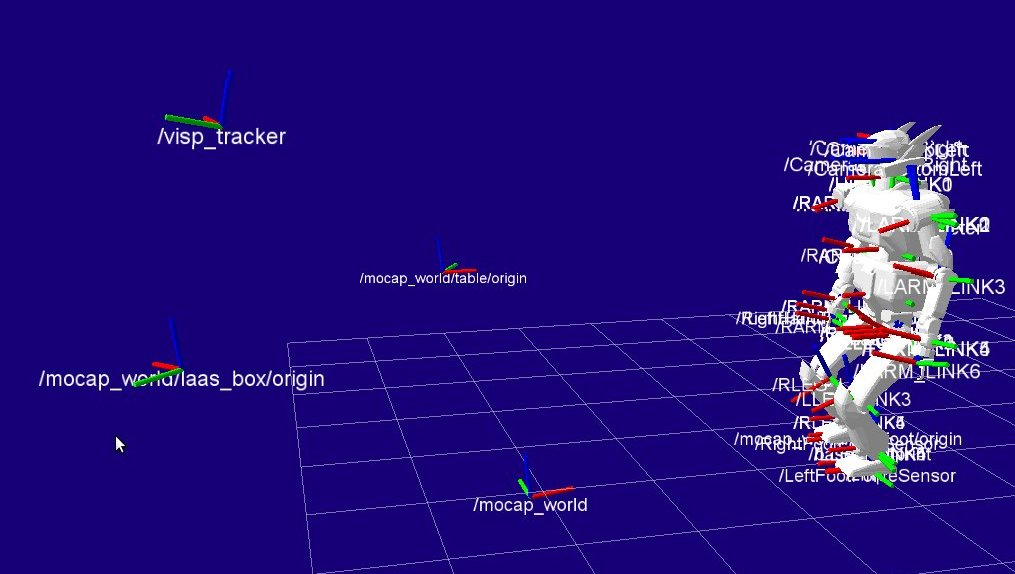
\includegraphics[width=.95\linewidth]{src/chap4-integration/rviz-full.jpg}
%    FIXME
%  \end{center}
%  \caption{Cycle de conception d'une architecture robotique. \label{fig:archidesign}}
%\end{figure}


Une fois validée en simulation, l'architecture est portée sur le robot
proprement dit. On peut alors faire tourner l'architecture sans
envoyer réellement les commandes aux actionneurs afin de vérifier
l'accès aux données capteurs, les délais induits par les
communications entre les hôtes, etc. Enfin, l'architecture peut être
testée réellement en validant plusieurs scénarii adaptés de difficulté
croissante. Une fois l'expérience validée, on peut alors changer
certains composants afin de tester de nouvelles stratégies ce qui fait
débuter un nouveau cycle.


\begin{figure}
  \begin{center}
    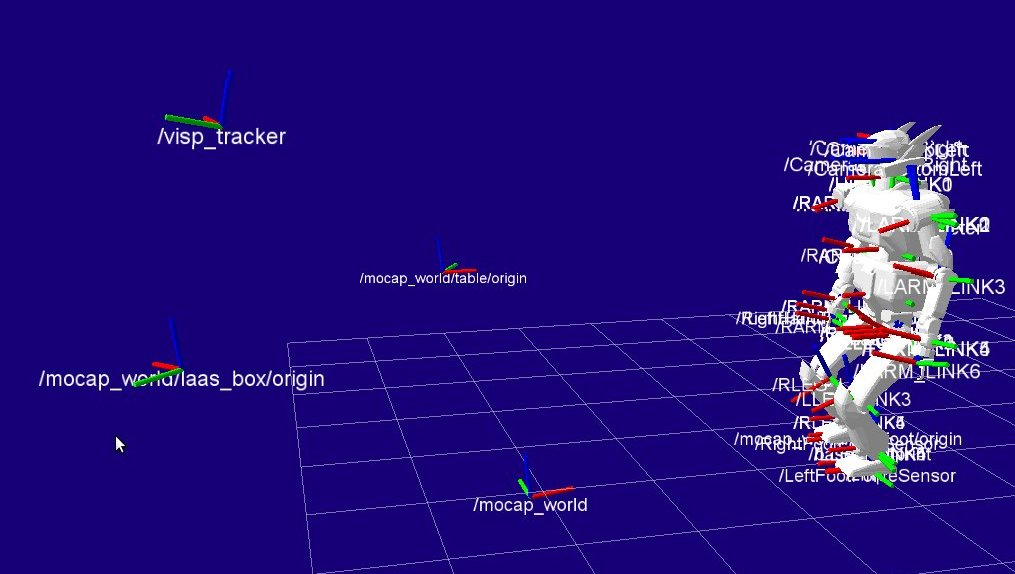
\includegraphics[width=.95\linewidth]{src/chap4-integration/rviz-full.jpg}
  \end{center}
  \caption{Architecture associant de nombreux composants
    robotiques intégrant le contrôleur du robot exécutant une tâche de
    locomotion, le système de capture de mouvement et le processus
    complet de vision utilisant l'algorithme de suivi décrit dans
    cette section pour estimer la position d'un cube.}
\end{figure}



\section{Conclusion}


Construire une architecture robotique est une tâche ardue, non
seulement parce qu'elle agrège des algorithmes complexes, mais surtout
parce qu'il est nécessaire de considérer la plate-forme utilisée et
les problèmes techniques qui lui sont propres -- délais, puissance de
calcul disponible --, afin de construire un ensemble
fonctionnel. Cette section a donc à la fois présenté comment
développer un composant robotique puis comment combiner plusieurs
composants pour réaliser une architecture. Les différentes difficultés
inhérentes à la conception d'un système ont été passées en revue ainsi
que les stratégies qui ont été adoptées au cours de ces trois
années. Il est probable qu'au cours des prochaines années de
nombreuses architectures robotiques voient le jour sur des robots
humanoïdes afin de les rendre sensibles à l'évolution de leur
environnement. Un objectif ambitieux pour lequel les robots mobiles
restent la plate-forme d'expérimentation principale dans l'état actuel
de la littérature.


